\documentclass[a4paper, 11pt]{scrartcl}
\usepackage[utf8]{inputenc}
\usepackage[czech]{babel}
\usepackage[unicode]{hyperref}
\usepackage{graphicx}
\usepackage{listings}
\usepackage{caption}

\DeclareCaptionType{ntscarea}[][Netscape Area]

\title{Historie prohlížeče Netscape}
\date{23. května 2014}
\author{Tomáš Havlík}

\begin{document}

\begin{titlepage}
\begin{center}

\includegraphics[scale=0.75]{ntsc_logo.png}~\\[1cm]
\textsc{\LARGE Historie Netscape}\\[0.5cm]
\textsc{\Large Vzestup a~pád nejzásadnějšího webového prohlížeče}\\[1cm]
\textsc{Tomáš Havlík\\23. května 2014}
\end{center}
\end{titlepage}

\newpage


\section{Počátky}
Historie prohlížeče Netscape sahá do roku 1992, kdy Marc Andreessen, student počítačových věd na Univerzitě v~Illinois, dal vzniknout společně s~kolegou prvnímu graf\/ickému webovému prohlížeči\footnote{Jednalo se o~první prohlížeč, který umožňoval zobrazovat obrázky v~interním okně. Prvním webovým klientem s~GUI je Erwise, vydaný v~dubnu 1992.} Mosaic. World Wide Webu byly v~té době pouhé dva roky a~sloužil především k~předávání informací v~akademické sféře.\\
Po dokončení prací na prohlížeči Mosaic se Marc přesunul do Silicon Valley a~zanedlouho založil společnost Mosaic Communications, později známou jako Netscape Communications Corporation. První beta verze prohlížeče Netscape spatřila světlo světa v~říjnu 1994, o~dva měsíce později pak vyšel finální produkt. Web se konečně stal masovou záležitostí.

\begin{ntscarea}[ht]
\begin{equation}
\xi = \int_{-1}^1 \! \left(\frac{4}{\cos 0^\circ}-x^2\right) \, \mathrm{d}x
\end{equation}
\caption{Aproximace plochy černé planetky v~logu Netscape při rozměru strany 2 jednotky.}
\end{ntscarea}


\section{Konkurence}
V~té samé době se však na oblast webu zaměřil i~jistý softwarový gigant – společnost Microsoft. Shodou okolností právě f\/inišoval vývoj nových Windows a~Bill Gates viděl v~internetu dokonalého společníka operačního systému. Redmondská společnost si licencovala Mosaic a~začala vyvíjet Internet Explorer (obr.~\ref{fig:one}).

\begin{figure}[ht]
\centering

\includegraphics[scale=1]{icons.png}
\caption{Ikonky vybízející ke stažení dvou navzájem konkurujících si prohlížečů.}
\label{fig:one}
\end{figure}

Microsoft tehdy také začal s~používáním proslule známých špinavých taktik. Dle slov Jamese Barksdale, tehdejšího vedoucího ředitele Netscape Communications, usiloval výrobce Windows o~zastavení prací na prohlížeči Netscape pro Windows 95 výměnou za ponechání relativně malého trhu, který zahrnoval ostatní operační systémy, plně v~rukou Netscapu.\cite{competing} Je vhodné zmínit, že webový prohlížeč Netscape Navigator byl v~této době dostupný na následujících platformách:

\begin{itemize}
\item Microsoft Windows 3.11, 95, NT
\item Mac OS
\item GNU/Linux
\item OS/2
\item Solaris
\end{itemize}

\newpage

Další strategií Microsoftu bylo podmanění si výrobců OEM\footnote{Original Equipment Manufacturer – výrobce zařízení, jež využívá komponenty jiných výrobců} počítačů. Těm bylo vyhrožováno, že pokud nahradí ikonu Internet Exploreru právě Netscape Navigatorem, bude jim odebrána licence na Windows 95.\cite{bbc} Internetový prohlížeč se tehdy stal nedílnou součástí tohoto operačního systému. Tyto kroky vyvrcholily v soudní proces s názvem United States v.~Microsoft Corp. který se zabýval zneužitím monopolního postavení na trhu internetových prohlížečů.

\section{Nadčasový produkt}
Netscape se však neohroženě řítil dál a~po raketovém nástupu v roce 1995 dosáhl svého vrcholu na grafech uživatelů těsně pod hranicí 80~\%. Nikdo tehdy netušil, že za deset let se bude stejný výkon opakovat, tentokrát však v~barvách Internet Exploreru.

\begin{figure}[ht]
\centering
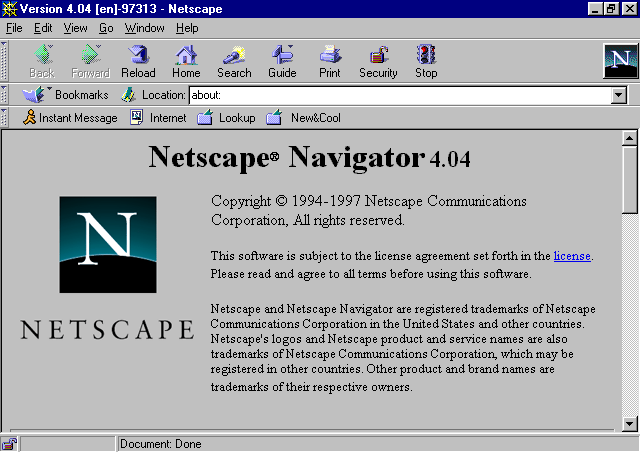
\includegraphics[scale=0.7]{ntsc.png}
\caption{Webový prohlížeč Netscape Navigator ve verzi 4.04 běžící pod Windows 95.}
\label{fig:two}
\end{figure}

Prohlížeč přinesl řadu vylepšení, některé z~nich můžeme vídat do dnešních dní. Kromě kontroverzního tagu \textless blink\textgreater{} se jedná například o~využití rámových elementů, jazyk JavaScript nebo podporu cookies. Od verze 3.0 se Netscape začal nabízet ve dvou verzích. Základní verze, nazvaná Standard Edition nebo také Netscape Navigator (obr.~\ref{fig:two}), obsahovala pouze webový prohlížeč. Gold Edition, později přejmenovaná na Netscape Communicator, pak obsahovala také e–mailový klient, čtečku diskuzních skupin a~WYSIWYG\footnote{What You See is What You Get – \uv{co vidíš, to dostaneš}} editor stránek.

\begin{figure}[ht]
\centering
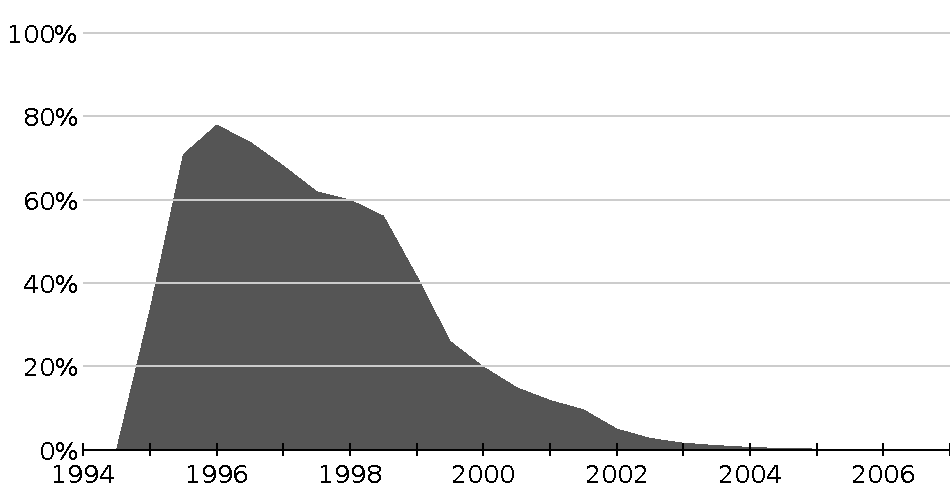
\includegraphics[scale=.8]{marketshare.pdf}
\caption{Tržní podíl prohlížečů z rodiny Netscape v letech 1994–2007}
\label{fig:three}
\end{figure}

\begin{table}[ht]
\centering
\begin{tabular}{|l|c|c|c|}
\hline
 & 1/98 & 3/98 & 6/98 \\
\hline
Netscape & 61~\% & 57~\% & 52~\% \\
\hline
Microsoft & 36~\% & 42~\% & 46~\% \\
\hline
\end{tabular}
\caption{Tržní podíl Netscape a Microsoftu v první polovině roku 1998.\cite{cnn}}
\label{tab:one}
\end{table}

Postupem času se však náskok Netscapu rapidně snižoval (obr.~\ref{fig:three}) a~na vedoucích příčkách jej v~roce 1998 nahradil Internet Explorer. Ten samý rok ztrátovou Netscape Communications Corporation odkoupila společnost America Online (AOL) za 4 miliardy dolarů.

\newpage

\section{Otevřená budoucnost}
Na počátku roku 1998 bylo rozhodnuto o~přepsání a~uvolnění kódu ke Communicatoru. Tentýž rok vzniklo renderovací jádro Gecko a~\uv{nástupnický} webový prohlížeč Mozilla\footnote{Složenina slov Mosaic a~Godzilla. Původně šlo o~jádro Netscape, následně dostal toto pojmenování nový webový prohlížeč z~dílny společnosti.}. Ten se postupem času oprostil o~nadbytečné funkce, a~jakožto samostatný prohlížeč Firefox vyrazil do druhé války browserů, kde o~deset let později vystřídal léta neohrožený Internet Explorer. Žezlo se tak alespoň na chvíli vrátilo do pařátů ještěra.

\begin{lstlisting}[language=C++,caption=Ukázka kódu Mozilly – výběr posledního uzlu v červeno–černé stromové struktuře.,captionpos=b]
nsNode* nsRBTree::Last(nsNode& aNode){
	nsNode* result=0;

	if(mRoot) {
		result=mRoot;
		while(result->GetRightNode()) {
			result=result->GetRightNode();
		}
	}
	return result;
}
\end{lstlisting}

\newpage

\begin{thebibliography}{}
\bibitem{competing}
CUSUMANO, Michael A. \textit{Competing on Internet Time: Lessons From Netscape And Its Battle With Microsoft.} Free Press, 2000. ISBN 978–0684863450.
\bibitem{bbc}
Netscape: A history. In \textit{BBC News World Edition} [online]. British Broadcasting Corporation, 2000 [cit. 23. května 2014]. Dostupné z: http://news.bbc.co.uk/2/hi/in\_depth/business/2000/microsoft/635689.stm
\bibitem{cnn}
Behind the numbers: Browser market share. In \textit{CNN Technology} [online]. Cable News Network, 1998 [cit. 23. května 2014]. Dostupné z: http://edition.cnn.com/TECH/computing/9810/08/browser.idg/
\end{thebibliography}

\end{document}
